\documentclass[12pt,a4paper]{article}

\usepackage[T1,T2A]{fontenc}
\usepackage[utf8]{inputenc}
\usepackage[english, russian]{babel}
\usepackage{indentfirst}
\usepackage{misccorr}
\usepackage{graphicx}
\usepackage{amsmath}
\usepackage{graphicx}
\usepackage{float}
\usepackage[left=20mm,right=10mm, top=20mm,bottom=20mm,bindingoffset=0mm]{geometry}

\setlength{\parskip}{6pt}
\DeclareGraphicsExtensions{.png}

\begin{document}

    \begin{titlepage}
        \begin{center}
            \large
            Санкт-Петербургский политехнический университет\\Петра Великого\\
            \vspace{0.5cm}
            Физико-механический институт\\
            \vspace{0.25cm}
            Высшая школа прикладной математики и вычислительной физики\\
            \vspace{0.25cm}
            \textbf{Прикладная математика и информатика}
            \vfill
            \textsc{\LARGE\textbf{Курсовая работа по теме:
            }}\\[5mm]
            \Large
            \textbf{"Применение индекса Жаккара для описания относительных размеров брусов при итерациях"}\\
            \vspace{0.5cm}
            по дисциплине "Интервальный анализ"
        \end{center}
        \vfill
        \begin{tabular}{l p{175} l}
            Выполнила студентка\\группы 5030102/80201 && Деркаченко Анна Олеговна
            \vspace{0.25cm}
            \\Проверил\\доцент, к.ф.-м.н. && Баженов Александр Николаевич
        \end{tabular}
        \vfill
        \begin{center}
            Санкт-Петербург\\2021 г.
        \end{center}
    \end{titlepage}

\newpage
\begin{center}
    \tableofcontents
    \setcounter{page}{2}
\end{center}
\newpage
\begin{center}
    \listoffigures
\end{center}

\newpage

\section{Постановка задачи}
Индекс Жаккара используется для сравнения множеств в различных проблемных областях. Но данный индекс можно обобщить на случай данных с интервальной неопределенностью и использовать для проверки их совместности.

Для иллюстрации применения индекса Жаккарда будем использовать задачи, рассмотренные в лабораторной, посвященной субдифференциальному методу Ньютона, то есть ИСЛАУ вида:
\begin{equation}
    \label{islau1}
    \begin{pmatrix}
        [3,4] & [5,6]\\
        [-1,1] & [-3,1]
    \end{pmatrix}
    \cdot{x}=
    \begin{pmatrix}
        [-3,3]\\
        [-1,2]
    \end{pmatrix}
\end{equation}

\begin{equation}
    \label{islau2}
    \begin{pmatrix}
        [3,4] & [5,6]\\
        [-1,1] & [-3,1]
    \end{pmatrix}
    \cdot{x}=
    \begin{pmatrix}
        [-3,4]\\
        [-1,2]
    \end{pmatrix}
\end{equation}

При решении обеих ИСЛАУ будем подсчитывать индекс Жаккара для каждой компоненты и проиллюстрируем зависимость размеров бруса на каждой итерации от предыдущих измерений.

\section{Теория}
\subsection{Субдифференциальный метод Ньютона}
Для начала вспомним, как организуется процесс решения ИСЛАУ субдифференциальным методом Ньютона.

\textbf{Построение итерационного процесса:}
\begin{equation}
    x^k=x^{k-1}-\tau(D^{k-1})^{-1}\mathcal{F}(x^{k-1}),
\end{equation}
где $\mathcal{F}(x)=sti\:(C\cdot{sti}^{-1}\:(x))-x+sti\:(d)$, $sti:\mathbb{KR}^n\rightarrow\mathbb{R}^{2n}$ - операция стандартного погружения, $D^{k-1}$ - субградиент отображения $\mathcal{F}$ в точке $x^{k-1}$, $\tau$ - константа (по умолчанию выбрана $\tau=1$).

\subsection{Индекс Жаккара}
Индекс Жаккара можно использовать для оперирования с относительными величинами. Например, для сопоставления допусков и размеров деталей, погрешности измерителей и значений измеряемых величин.

Исходный индекс Жаккара имеет вид:
\begin{equation}
    J(A,B)=\frac{n(A\cap{B})}{n(A\cup{B})},
\end{equation}
где $n$ - некоторая мера множеств (например, мощность).

Обобщим данный индекс для подсчета степени совместности двух интервалов $\textbf{x},\textbf{y}:$
\begin{equation}
    |Rwid(\textbf{x},\textbf{y})|=\frac{wid(\textbf{x}\wedge\textbf{y})}{wid(\textbf{x}\vee\textbf{y})}
\end{equation}
\newpage
\textbf{\textit{Свойства Rwid:}}
\begin{itemize}
    \item если $\textbf{x}\cap\textbf{y}\not=\varnothing$, то $Rwid(\textbf{x},\textbf{y})\geq0$
    \item иначе $Rwid(\textbf{x},\textbf{y})<0$
    \item если $\textbf{x}$ и $\textbf{y}$ пересекаются в одной точке, то $Rwid(\textbf{x},\textbf{y})=0$
    \item если $\textbf{x}=\textbf{y}$, то $Rwid(\textbf{x},\textbf{y})=1$
    \item если $x\not=y\in\mathbb{R}$, то $Rwid(x,y)=-1$
\end{itemize}

Таким образом, $-1\leq{Rwid(\textbf{x},\textbf{y})}\leq1$. При этом отрицательность индекса Жаккара свидетельствует об несовместности данных, а само значение индекса - о степени несовместности данных.

В случае многомерности данных используется следующее обобщение индекса Жаккара:
\begin{equation}
    Rwid_k(\textbf{x},\textbf{y})=\frac
    {min\{\overline{\textbf{x}_k},\overline{\textbf{y}_k}\}-max\{\underline{\textbf{x}_k},\underline{\textbf{y}_k}\}}
    {max\{\overline{\textbf{x}_k},\overline{\textbf{y}_k}\}-min\{\underline{\textbf{x}_k},\underline{\textbf{y}_k}\}},
\end{equation}
где $\textbf{x}=\{x_k\},\textbf{y}=\{y_k\},k$ - номер компоненты. Данный индекс подсчитывается для каждой из компонент отдельно.

\section{Реализация}
Реализация курсовой работы проводилась с помощью встроенных средств в среде разработки Octave, библиотеки kinterval для полной интервальной арифметики.

Исходный код лабораторной работы размещен в GitHub-репозитории.

URL: https://github.com/derkanw/IntervalAnalysis/tree/main/coursework

\section {Результаты}
Начальный брус обозначен синим цветом, конечный вид бруса - красным, зеленой пунктирной линией - границы допускового множества.

Индекс Жаккара будем подсчитывать относительно двух последовательных итераций метода Ньютона покомпонентно.

\subsection{Решение задачи \eqref{islau1}}
Решение задачи \eqref{islau1} с параметром $\tau=1$ получено за 4 итерации: $x=
\begin{pmatrix}
    [-1.4803*10^{-16},0.5]\\
    [-0.5,0.1667]
\end{pmatrix}$

\begin{figure}[H]
    \centering
    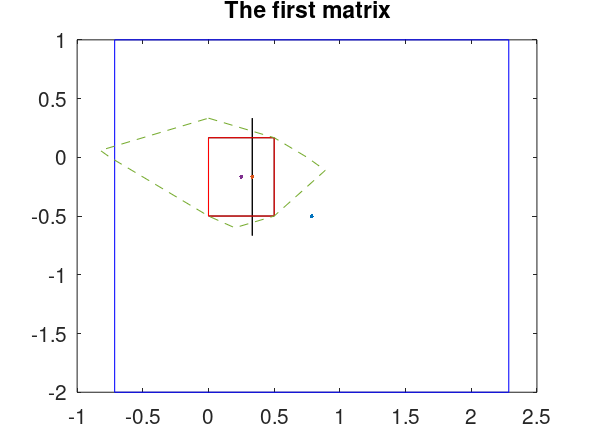
\includegraphics[scale=0.6]{Images/matrix1.png}
    \caption{Иллюстрация брусов при решении задачи \eqref{islau1}}
\end{figure}

\begin{table}[H]
    \centering
    \begin{tabular}{|c|c|c|c|c|}
        \hline
        k & $x_1$ & $x_2$ & $rwid_1$ & $rwid_2$\\\hline
        1 & [2.2857,-0.71429] & [-2,1] & - & -\\\hline
        2 & [0.33333,0.33333] & [-0.66667,0.33333] & 0 & 0.3333\\\hline
        3 & [2.2204e-16,0.5] & [-0.5,0.16667] & 0 & 0.6667\\\hline
        4 & [-1.4803e-16,0.5] & [-0.5,0.16667] & 1 & 1\\\hline
    \end{tabular}
    \caption{Итерационный процесс решения задачи \eqref{islau1}}
\end{table}

\begin{figure}[H]
    \centering
    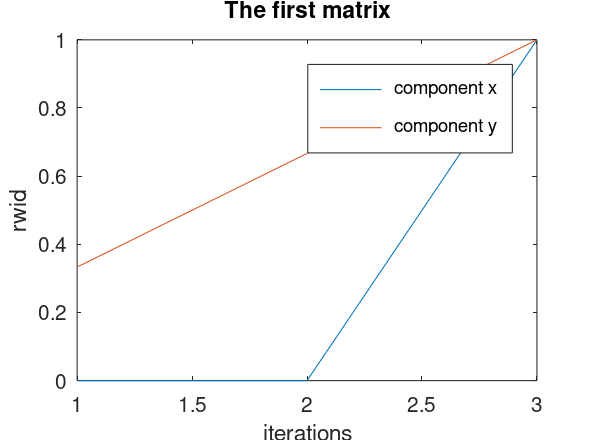
\includegraphics[scale=0.6]{Images/rwid1.png}
    \caption{Индекс Жаккара при решении задачи \eqref{islau1}}
\end{figure}

\subsection{Решение задачи \eqref{islau2}}
При решении \eqref{islau2} с параметром $\tau=1$ конечное решение не имеет возмости получить, поэтому было рассмотрено 20 показательных итераций.
Решение данной ИСЛАУ, полученное на 20 итерации, равно $x=
\begin{pmatrix}
    [-0.3333,1]\\
    [-0.3333,0]
\end{pmatrix}$

\begin{figure}[H]
    \centering
    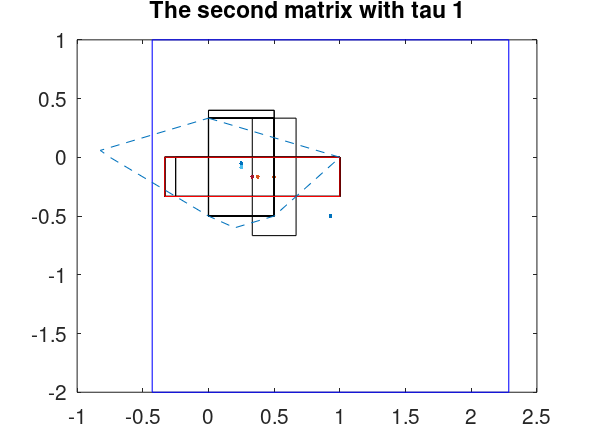
\includegraphics[scale=0.6]{Images/matrix2.png}
    \caption{Иллюстрация брусов при решении задачи \eqref{islau2} с $\tau=1$}
\end{figure}

Приведем некоторые значения из вычислений:
\begin{table}[H]
    \centering
    \begin{tabular}{|c|c|c|c|c|}
        \hline
        k & $x_1$ & $x_2$ & $rwid_1$ & $rwid_2$\\\hline
        1 & [2.2857,-0.42857] & [-2,1] & - & -\\\hline
        2 & [0.33333,0.66667] & [-0.66667,0.33333] & 0 & 0.3333\\\hline
        3 & [-0.33333,1] & [-0.33333,5.5511e-17] & 0.25 & 0.3333\\\hline
        4 & [2.2204e-16,0.5] & [-0.5,0.33333] & 0.375 & 0.4\\\hline
        5 & [-0.33333,1] & [-0.33333,-5.5511e-17] & 0.375 & 0.4\\\hline
        6 & [-1.1102e-16,0.5] & [-0.5,0.4] & 0.375 & 0.3704\\\hline
        7 & [-0.25,1] & [-0.33333,-5.5511e-17] & 0.4 & 0.3704\\\hline
        8 & [-1.1102e-16,0.5] & [-0.5,0.4] & 0.4 & 0.3704\\\hline
        9 & [-0.25,1] & [-0.33333,0] & 0.4 & 0.3704\\\hline
        10 & [1.1102e-16,0.5] & [-0.5,0.33333] & 0.4 & 0.4\\\hline
        11 & [-0.33333,1] & [-0.33333,0] & 0.375 & 0.4\\\hline
        12 & [1.6653e-16,0.5] & [-0.5,0.33333] & 0.375 & 0.4\\\hline
    \end{tabular}
    \caption{Итерационный процесс решения задачи \eqref{islau2}}
\end{table}
В последующих итерациях индекс Жаккара не меняет своего значения.

\begin{figure}[H]
    \centering
    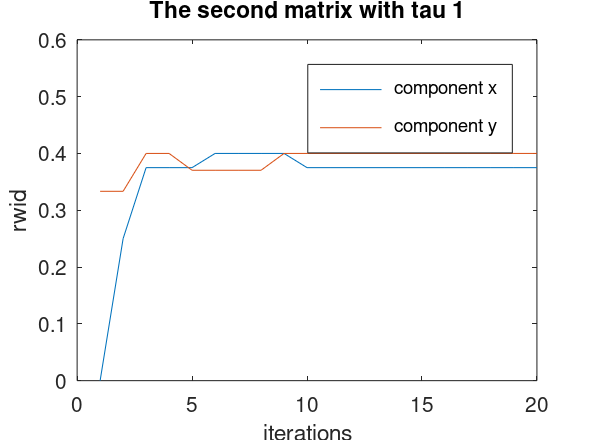
\includegraphics[scale=0.6]{Images/rwid2.png}
    \caption{Индекс Жаккара при решении задачи \eqref{islau2}}
\end{figure}

\subsection{Решение задачи \eqref{islau2} с уменьшенным параметром $\tau$}
Если положить значение $\tau=0.1$ при решении задачи \eqref{islau2}, можно выделить решение, полученное на 100 итерации, $x=
\begin{pmatrix}
    [-0.15971,0.8195]\\
    [-0.39354,0.12034]
\end{pmatrix}$

\begin{figure}[H]
    \centering
    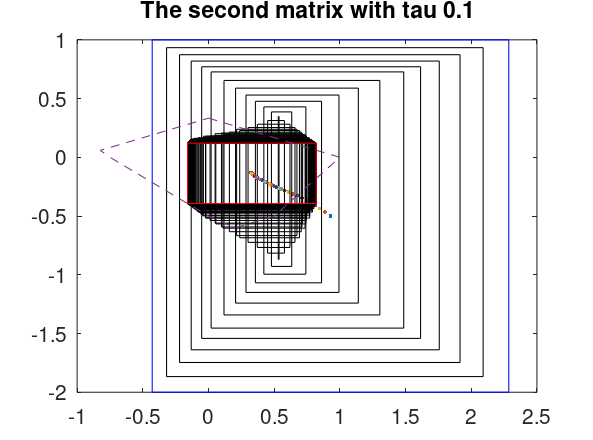
\includegraphics[scale=0.6]{Images/matrix3.png}
    \caption{Иллюстрация брусов при решении задачи \eqref{islau2} с $\tau=0.1$}
\end{figure}

Приведем некоторые значения из вычислений:
\begin{table}[H]
    \centering
    \begin{tabular}{|c|c|c|c|c|}
        \hline
        k & $x_1$ & $x_2$ & $rwid_1$ & $rwid_2$\\\hline
        1 & [2.2857,-0.42857] & [-2,1] & - & -\\\hline
        2 & [2.0905,-0.31905] & [-1.8667,0.93333] & 0 & 0.9333\\\hline
        3 & [1.9148,-0.22048] & [-1.7467,0.87333] & 0 & 0.9357\\\hline
        4 & [1.7566,-0.13176] & [-1.6387,0.81933] & 0 & 0.9382\\\hline
        5 & [1.6143,-0.051919] & [-1.5415,0.77073] & 0 & 0.9407\\\hline
        6 & [1.4862,0.01994] & [-1.454,0.72699] & 0 & 0.9432\\\hline
        7 & [1.3042,0.11795] & [-1.3419,0.65429] & 0 & 0.9153\\\hline
        8 & [1.1405,0.20615] & [-1.2411,0.58886] & 0 & 0.9167\\\hline
        9 & [0.9931,0.28554] & [-1.1503,0.52998] & 0 & 0.9182\\\hline
        10 & [0.86046,0.35698] & [-1.0686,0.47698] & 0 & 0.9198\\\hline
        11 & [0.74108,0.42128] & [-0.99507,0.42928] & 0 & 0.9216\\\hline
        12 & [0.63364,0.47916] & [-0.92889,0.38635] & 0 & 0.9234\\\hline
        13 & [0.53694,0.53124] & [-0.86934,0.34772] & 0 & 0.9253\\\hline
        14 & [0.44991,0.57812] & [-0.81574,0.31295] & 0 & 0.9274\\\hline
        15 & [0.37159,0.6203] & [-0.7675,0.28165] & 0.5155 & 0.9295\\\hline
        16 & [0.3011,0.65827] & [-0.72408,0.25349] & 0.6963 & 0.9318\\\hline
        17 & [0.23765,0.69245] & [-0.68501,0.22814] & 0.7854 & 0.9341\\\hline
        18 & [0.21389,0.6732] & [-0.66651,0.23866] & 0.9101 & 0.9686\\\hline
        19 & [0.15917,0.70588] & [-0.63319,0.21479] & 0.8401 & 0.9368\\\hline
        20 & [0.10992,0.73529] & [-0.6032,0.19331] & 0.8742 & 0.9393\\\hline
        21 & [0.098925,0.71176] & [-0.59288,0.20731] & 0.9458 & 0.9216\\\hline
    \end{tabular}
    \caption{Итерационный процесс решения задачи \eqref{islau2} с $\tau=0.1$}
\end{table}
В последующих итерациях индекс Жаккара колеблется в пределах величины $0.95$ для обеих компонент.

\begin{figure}[H]
    \centering
    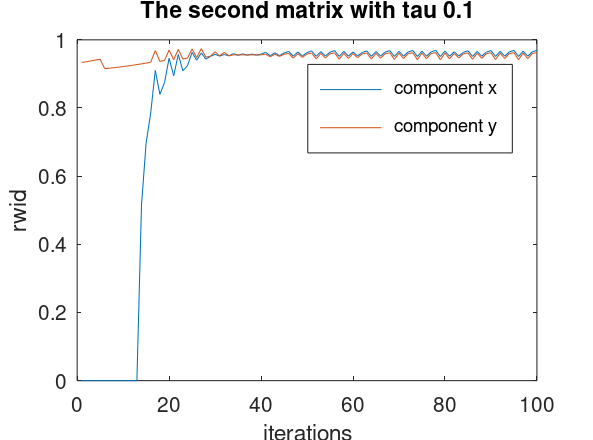
\includegraphics[scale=0.6]{Images/rwid3.png}
    \caption{Индекс Жаккара при решении задачи \eqref{islau2} с $\tau=0.1$}
\end{figure}

\section{Обсуждение}
\subsection{Решение задачи \eqref{islau1}}
При построении итерационного процесса для задачи \eqref{islau1} наблюдается вырожденность в линию бруса на второй итерации, о чем свидетельствует индекс $Rwid_1=0$, так как первая компонента выродилась в точку. Положительные значения $Rwid_2<1$ говорит о сходимости по второй компоненте. При этом на 4 итерации значения индекса Жаккара, равные 1 для каждой компоненты, показывают, что процесс решения данной задачи достиг точного решения.

Данный пример не совсем хорошо иллюстрирует все особенности применения индекса Жаккара для характеризации итерационного процесса из-за слишком быстрой сходимости метода для указанной ИСЛАУ.

\subsection{Решение задачи \eqref{islau2}}
По заданному ИСЛАУ невозможно достичь точного решения, поэтому индекс Жаккара не принимает нигде значения, равного единице. При этом процесс сходимости на некоторых начальных итерациях и последующих итерациях, начиная с 12, останавливается, и значения $Rwid$ для обоих компонент перестают изменяться, но показывают некоторую степень совместности размеров брусов. Данное значение достаточно отличается от единичного, поэтому можно сделать вывод, что полученные брусы не очень точно описывают искомое решение ИСЛАУ. Так же интересно заметить постоянное чередование одних и тех же размеров брусов. Все это свидетельствует о необходимости произвести модификацию параметров метода.

По этой причине был рассмотрен параметр $\tau=0.1$. Для данной задачи так же не было получено значения $Rwid=1$ для каждой из компонент, то теперь индекс Жаккара уже с 21 итерации для обоих компонент находится в пределах $0.95$ и не выходит за них в течении всего процесса. Это демонстрирует, что произошло достаточно хорошее уточнение решения для заданной ИСЛАУ. Большое количество нулей в начале итераций по первой компоненте можно объяснить неверностью построения интервалов для брусов, что корректируется в процессе работы метода Ньютона после 15 итерации. При этом на итерациях 15-21 значения $Rwid$ для первой компоненты возрастают, что характеризиует увеличение бруса решения, то есть происходит грубая локализация решения. После 21 итерации для первой компоненты и на всех итерациях для второй компоненты заметно медленное уточнение данной локализации, и брусы решения уже являются подмножествами брусов, полученных на этапе грубой локализации.

\section{Краткий вывод}
Данное обобщение индекса Жаккара на случай интервальных данных отражает этапы итерационного процесса рассматриваемой ИСЛАУ. В общем случае можно выделить такие этапы:
\begin{enumerate}
    \item Идет сходимость по компонентам, чьи собственные числа имеют значения, меньшее 1
    \item Для остальных компонент происходит этап грубой локализации области решения (увеличение бруса) - величина индекса Жаккара увеличивается
    \item Далее происходит уточнение брусов в границах выделенной области локализации решения - индекс Жаккара начинает уменьшаться
    \item Процесс медленно сходится к решению с некоторой точностью - индекс Жаккара становится примерно равным 1
\end{enumerate}

\begin{thebibliography}{1}
    \bibitem{}
    А.Н.Баженов. Мера (функционал) совместности интервальных величин для применения в
    анализе данных с интервальной неопределённостью. (Обобщение меры Жаккара). Санкт-Петербург, 2022.
\end{thebibliography}
\end{document}
